\subsubsection{Approximate Q-Learning}

Since there are a total of $5^{32}\approx10^{22}$ states, it is not possible to visit all as long as store all states during training. So we introduce the approximate Q-learning to avoid the side effects of unvisited states.

Our experience is summed up in a few powerful numbers. We take the following experimental value functions for approximate Q-values.

\begin{equation}
f_1(s, a) = \left\{\begin{aligned}
10 &, \text{if the WHITE side wins}\\
-10 &, \text{if the BLACK side wins}\\
0&,  \text{otherwise}\\
\end{aligned}\right. \\
\end{equation}
$$f_2(s,a)=N_{\text{our-survived}}  +\ 2*N_{\text{our-kings}}$$
all $N$ are numbers for state $s$

\begin{equation}
    f_3(s, a) = \sum\limits_{\text{our non-king pieces}\in s}\frac{1}{L_{\text{dis-to-bottom}}}
\label{f3}
\end{equation}
all $L$ are depth for state $s$

$$
f_4(s,a) = \sum\limits_{\text{our pieces}\in s}\frac{1}{min(L_{\text{dis-to-left}}, L_{\text{dis-to-right}})+1}
$$

Where $N$ means the number of pieces, and $L$ means the distance between the selected piece and the target line. All former formulas are only considered the state $s$.

We also need to take the state after the transition into consideration, by setting
$$f_5(s,a) = -f_1(s,a)$$
$$f_6(s,a)=N_{\text{opponent-survived}} + 2 * N_{\text{opponent-kings}}$$
all $N$ are numbers for state $s'$

\begin{equation}
    f_7(s, a) = \sum\limits_{\text{our non-king pieces}\in s'}\frac{1}{L_{\text{dis-to-bottom}}}
\end{equation}
all $L$ are depth for state $s'$

$$
f_8(s,a) = \sum\limits_{\text{our pieces}\in s'}\frac{1}{min(L_{\text{dis-to-left}}, L_{\text{dis-to-right}})+1}
$$

With the constructed value functions for approximate Q-values above, we could train with the method of approximate Q-learning:

$$sample = \sum_{i=1}^8w_if_i(s,a)$$
$$difference = sample - Q(s,a)$$
$$Q(s,a) \gets (1 - \alpha)Q(s,a) + \alpha (sample)$$
$$w_i \gets w_i + \alpha (difference)f_i(s,a)$$

For the training details, we set the discount factor $\gamma=0.8$, and all weights $w_i$ are initially set to be $10$. We firstly pre-train the model, we totally trained $3000$ epochs, with a learning rate to be $0.01$, and after the $1000$-th epoch, the learning rate times $0.99$ after each epoch. The opponent to be the minimax search with depth $3$.

Then we do finetune for the pre-trained model, similar to the pre-training, but we set the learning rate to be $0.001$ at initial, and the opponent to be the minimax search with depth $5$.

After finetuning, we tested the winning rate for our trained approximate Q-learning model, the winning rate has a great increase compared to the pretraining model. The winning rate of Approximate Q-learning and random increases from $89\%$ increase to $91\%$.

% ------------------------------------
\subsubsection{Neural Network}

Since testing the Minimax algorithm could generate a large amount of battle information, we want to make good use of it. By using the previous battle information to train a Neural Network, and generate a new feature for the \textbf{Approximate Q-learning}.

We collected the training data by storing the match information during testing the winning rate between Minimax with depth $7$ and another Minimax with depth $7$.
We store each board's information and the turn of the player during the matching. After matching, the board that was generated by the winner is set to have the label $+1$, and the board that was generated by the loser is set to have the label $-1$. Also, the board's generator was also recorded.

With the generated data, we could do training and inference to generate the new feature for approximate Q-learning.

\begin{figure}[t]
    \centering
    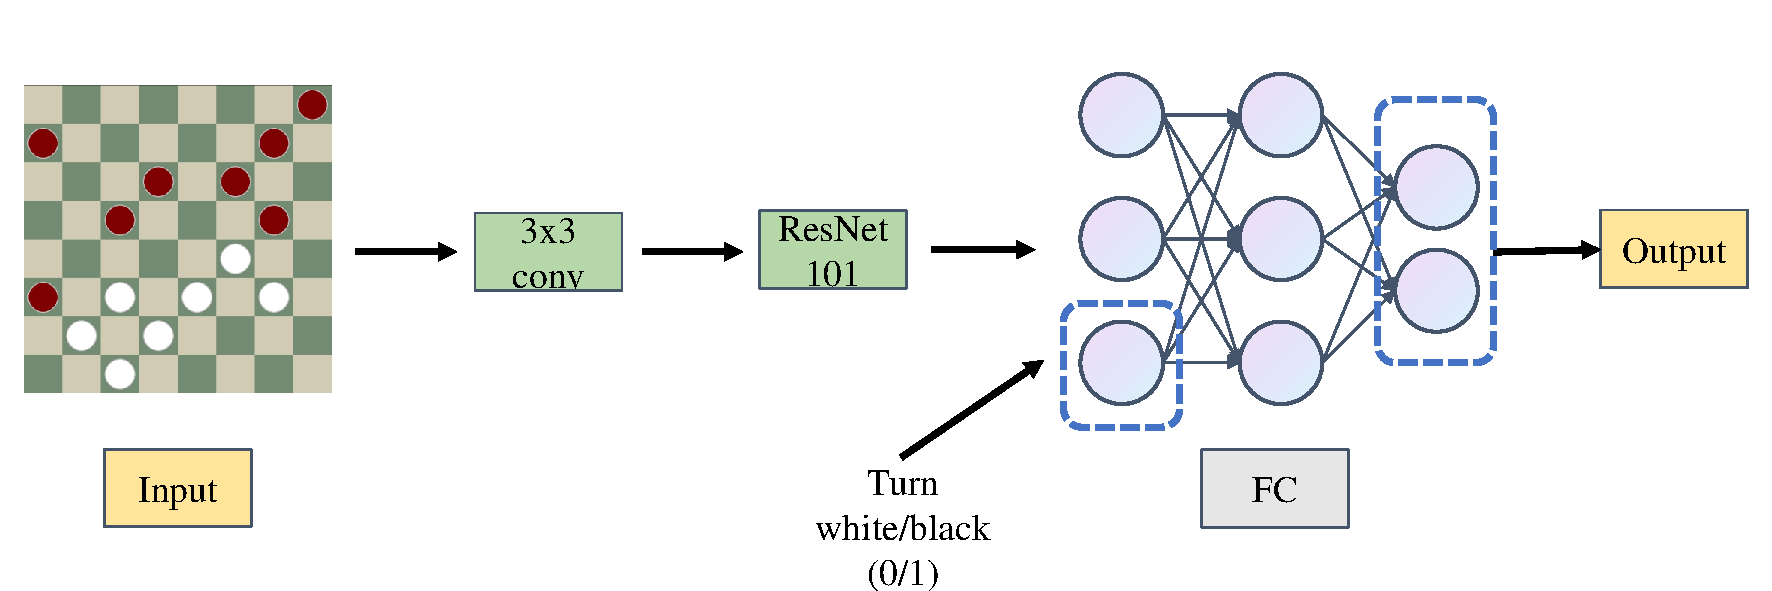
\includegraphics[width=\linewidth]{figures/neural.pdf}
    \caption{The pipeline of the Neural Network to generate new features.}
    \label{fig:pipeline}
\end{figure}

\begin{enumerate}
    \item \textbf{Training}
    Throw our observation during the matchings, almost all capture operations happened within $2$ steps. This means that in nearly all situations if a piece eats the opponent's pieces, it will not eat more than $2$ pieces. So if we consider the board as an image, a convolution kernel with $5\times 5$ receptive field is enough.

    After the convolution layer, we set ResNet101 and a $3$-layer fully connected MLP to do the $ 2$ classification task. The output layer includes two numbers since we are doing the $ 2$ classification, so the final output $+1$ or $-1$ is the prediction of the new state's winning rate. And we set this to be the new feature for approximate Q-learning.
    
    The total pipeline is shown in \ref{fig:pipeline}.
    
    \item \textbf{Inference} To generate the new feature, we put the origin board $s$, and the board $s'$ after action $a$ respectively into the network, and infer the winning rate. The winning rates are set to be the new feature $f_{new}(s,a)$.

\end{enumerate}

After generating the new feature, we put it into the original \textbf{Approximate Q-learning}, all settings are the same instead of adding a feature. And we could see that the winning rate has increased. The details are shown in Section \textbf{Result}.